\section{The MICE Experiment}
\label{sec:MICE}
  \subsection{Overview}
  \label{subsec:Overview}
  The Muon Ionization Cooling Experiment (MICE) will perform a practical demonstration of muon ionization cooling. Cooling refers to a reduction in the emittance of a beam, that is, the reduction of the phase-space volume occupied by the beam. Beam cooling is required for any future facility based on high intensity muon beams, such as a Neutrino Factory~\cite{ISS-Physics}, the ultimate tool to study leptonic CP-invariance violation, or a Muon Collider~\cite{MC_Overview}, a potential route to multi-TeV lepton -- anti-lepton collisions. Muon beams are generated via pion decay, and therefore have a large emittance, which must be reduced so that a reasonable fraction of the beam will fall within the acceptance of the downstream acceleration system.

  The short muon lifetime requires fast beam cooling that traditional techniques are unable to provide.  Ionization cooling was proposed in the early 1970s~\cite{Skrinsky, Neuffer}, but has not yet been demonstrated at the energies of interest for the Neutrino Factory or Muon Collider.  Ionization cooling reduces emittance by passing a beam through some suitable material of low atomic-number such as liquid hydrogen.  This leads to the reduction of all components of momentum due to ionization energy loss. Low atomic number absorbers are preferred because they minimise multiple scattering which ``heats'' the beam. %After the absorber, momentum is restored in the longitudinal direction only by means of radio frequency cavities.  The sequence is repeated leading to an overall reduction in the transverse phase-space occupied by the beam.

  \begin{figure}[bht]
    \begin{center}
      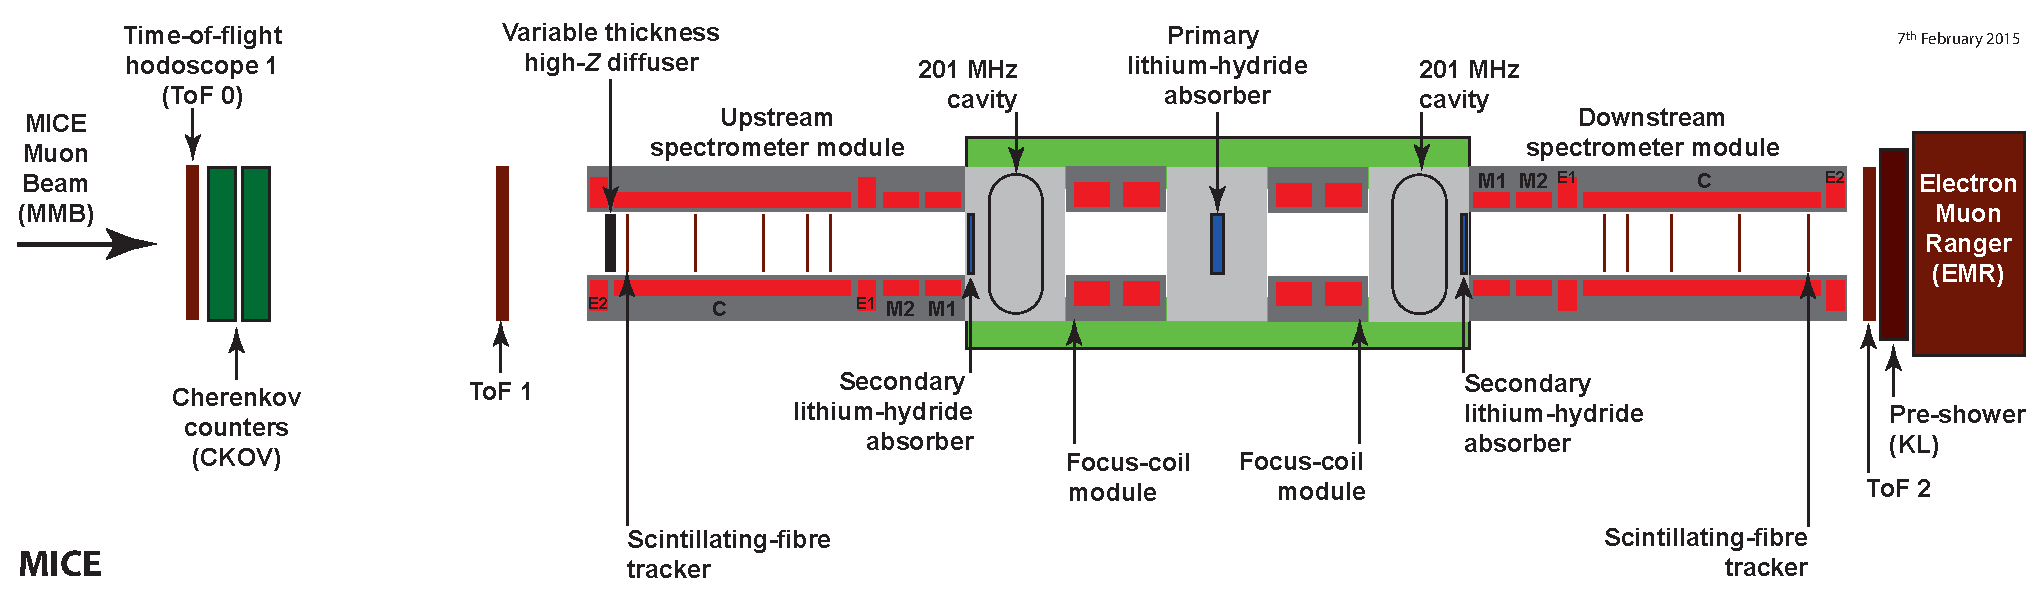
\includegraphics[width=1.0\linewidth]{01-MICE/Cooling-demo-labels.pdf}
      \caption{\label{fig:CoolingChannel} The beam diagnostics and cooling cell (indicated in green). $M$ refers to matching coils, $E$ to end coils and $C$ to the coils used to generate the solenoidal fields for tracking. Particle identification is provided by three time-of-flight stations, two threshold Cherenkov detectors and a downstream calorimeter composed of a pre-shower detector and electron-muon ranger. Emittance is measured upstream and downstream of the cooling cell by spectrometers. A diffuser is used to artifically increase the beam emittance prior to the cooling cell. Ionization energy loss occurs as the beam passes through the absorber modules, while longitudinal reacceleration is providing by radio frequency electric field cavities.}
    \end{center}
  \end{figure}

  MICE is sited at the Science and Technology Facilities Council Rutherford Appleton Laboratory in the U.K. and exploits the ISIS proton synchrotron to generate the muon beam~\cite{MiceTarget}.  The MICE beam line is described in detail in~\cite{BeamlineJINST}. A schematic of the full MICE experiment is shown in figure~\ref{fig:CoolingChannel}. The beamline is instrumented with with two threshold Cherenkov detectors, three time-of-flight (TOF) stations and a downstream calorimeter. The cooling cell consists of three absorber modules and two radio frequency (RF) cavities. Two high-precision trackers in a solenoidal field are used to measure the emittance change (see section~\ref{subsec:Trackers}).

  MICE is a staged experiment, that is, built and run in distinct steps. The first step of the programme, consisting of the muon beam line with particle identification, is now complete and results available in~\cite{BeamlineJINST, BeamCharacterisationEurPhysJ, EMRJINST, PionContaminationJINST}. The present step of the program, which introduced the trackers and the first absorber module, began taking data in 2015. % The demonstration of sustainable cooling, which includes longitudinal re-acceleration, will begin data taking in 2018.

%   \begin{figure}[tb]
%     \begin{center}
%       \includegraphics[width=0.75\linewidth]{01-MICE/BeamLineDEMOSans.pdf}
%       \caption{\label{fig:Beamline}The MICE Muon Beamline. A pion production target intercepts the protons of the circulating ISIS beam. Some of the subsequent pions are then captured by quadrupoles and guided down the beam line, passing through various PID detectors along the way, before delivery to the cooling cell itself. Emittance is measured immediately before and after the cooling cell using the scintillating fibre trackers.}
%       \end{center}
%   \end{figure}

  \subsection{The Scintillating Fibre Trackers}
  \label{subsec:Trackers}
  MICE is equipped with two identical, high precision scintillating-fibre (``scifi'') trackers, described in~\cite{TrackersNIM}. Each tracker is placed in a superconducting solenoid that provides a uniform field over the tracking volume. One tracker, TKU, is upstream of the cooling cell, the other, TKD, downstream.  Each tracker consists of 5 detector stations, labelled 1 to 5, as illustrated in figure~\ref{fig:Trackers}. TKU is orientated such that Station~5 sees the beam first, TKD is rotated by 180$^\circ$ such that Station~1 sees the beam first, thus, in both trackers, Station~1 is always nearest to the cooling cell (see figure~\ref{fig:CoolingChannel}).
 

  Each station is formed of three planes of 350~$\mu$m scintillating fibres, orientated at 120 degrees to one another. The fibres in each plane are arranged in two layers offset with respect to each other (a ``doublet layer''), in order to give 100$\%$ coverage of the plane area as illustrated in figure~\ref{fig:DoubletLayer}. The doublet layer is glued on to a sheet of mylar. The fibres are collected into groups of seven for readout, each group forming a single channel, as illustrated in figure~\ref{fig:DoubletLayer}b. The planes, also known as views, are labelled $U$, $V$ and $W$. Plane $U$ is attached to the station frame directly, plane $W$ on to plane $U$, and plane $V$ on to plane $W$. The fibre-plane orientations are illustrated in figure~\ref{fig:FibrePlaneOrientation}. Each station is oriented such that the fibres in the $U$ plane are vertical. The fibres produce scintillation light when ionizing radiation passes through them. Clear-fibre light guides transport the scintillation light to visible light photon counters (VLPCs) that are operated at 9~$K$ in a cryostat~\cite{TrackersNIM}. The signal from the VLPCs is digitised using front-end electronics developed by the D0 experiment~\cite{D0}. See~\cite{TrackersNIM} for details.
  
  \begin{figure}[tb]
    \centering
    \includegraphics[width=0.5\linewidth]{01-MICE/TrackerFrame.pdf} \hspace{2pc}%
    \includegraphics[width=0.35\linewidth]{01-MICE/TrackerPhoto.pdf}
    \caption{\label{fig:Trackers} Left: A schematic of the tracker carbon-fibre frame, showing the detector station positions.  The fibre planes are glued on to the upstream edge of the carbon-fibre station frames (shown in green). The longitudinal coordinate of the tracker coordinate system ($z_t$) increases as one moves from the fibre plane towards the station frame to which it is attached.  Right: A photograph of a tracker. The colour is due to the filtered lighting needed to protect the scintillating fibres. The intersecting lines visible on the station faces indicate the direction of the fibres in each plane.}
  \end{figure}

  \begin{figure}[tb]
    \begin{center}
      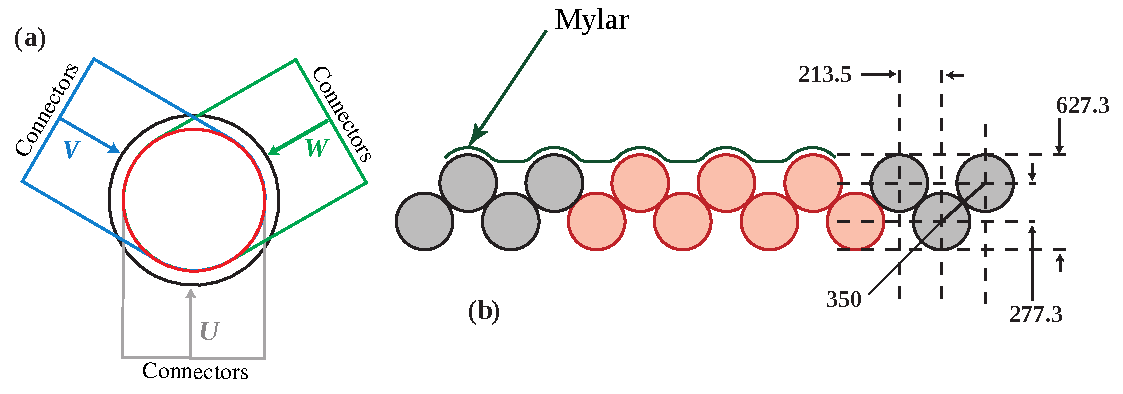
\includegraphics[width=0.85\textwidth]{01-MICE/doublet-layer.pdf}
      \caption{\label{fig:DoubletLayer}(a) Arrangement of the doublet layers in the scintillating fibre  stations. The outer circle shows the solenoid bore while the inner circle shows the limit of the active area of the tracker. The arrows indicate the direction that the individual 350\,$\mu$m fibres run. (b) Detail of the arrangement of the scintillating fibres in a doublet layer. The fibre spacing and the fibre pitch are indicated on the right-hand end of the figure in \,$\mu$m. The pattern of seven fibres shown in red form a single channel, which is readout via a clear-fibre light-guide. The sheet of mylar glued to the doublet layer is indicated. }
    \end{center}
  \end{figure}

  \begin{figure}[tb]
    \centering
    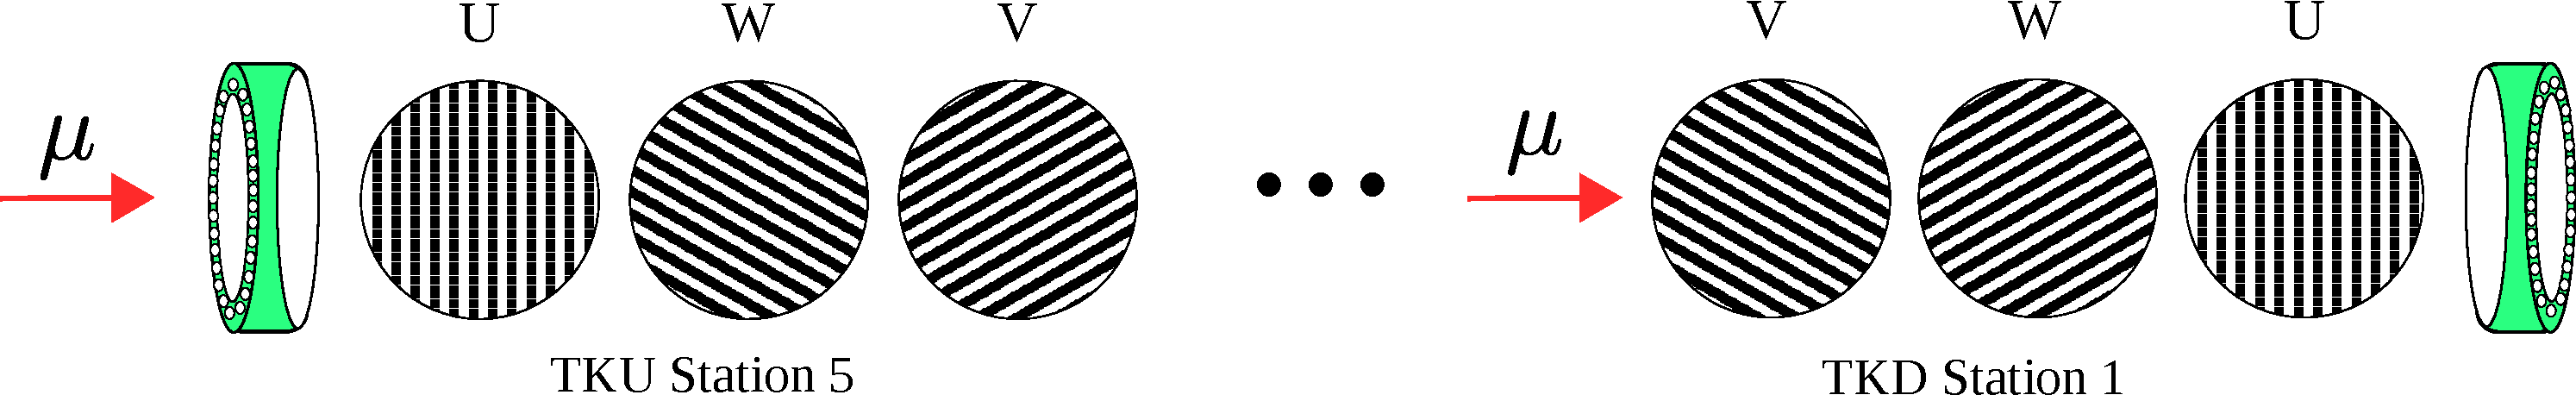
\includegraphics[width=0.95\linewidth]{01-MICE/FibrePlaneOrientation.pdf} \hspace{2pc}%
    \caption{\label{fig:FibrePlaneOrientation} The orientation of the fibres in each plane, as seen by the incoming beam, for both trackers. The green object is the station frame.}
  \end{figure}